\clearpage
\hypertarget{conBran vis}{}
\subsection{Branching with statement nodes}
\visHeader

\begin{itemize}

\item[$\blacktriangleright$] Currently, there is no method to help us initialize \texttt{box} from its pristine state (no partitions). Create one by editing
your metamodel (the \texttt{LearningBoxLanguage} diagram) and invoking the \texttt{Operations} dialogue by first selecting \texttt{Box}, then pressing
\texttt{F10}.\footnote{To review creating new operations, review Section 2.6 of Part II}

\item[$\blacktriangleright$] Name the new method \texttt{initializeBox} and, recalling the one rule of conditional branching, set its return type to
\texttt{EBoolean}.

\item[$\blacktriangleright$] Save and close the dialogue, then re-open the \texttt{grow} SDM and \emph{Quick Create} a new activity node from
\texttt{addNewPartition}.

\item[$\blacktriangleright$] This will be the node we'll use to invoke our helper method. Double click the node to invoke its properties editor and switch the
\texttt{Type} to a \texttt{StatementNode}. Name it \texttt{initialize} (Fig.~\ref{ea:newStatementNode}).

\item[$\blacktriangleright$] Before closing the dialogue, switch to the \texttt{Statement} tab, and create a \texttt{MethodCallExpression} to invoke your newest
method (Fig.~\ref{ea:statementMCE}). We want to access the \texttt{Box} object (\texttt{this}) and its \texttt{initalizeBox} method. It doesn't require any
parameters, so leave the values field empty. 

\begin{figure}[htbp]
   \centering
      \subfloat[Create a new \emph{StatementNode}]{
        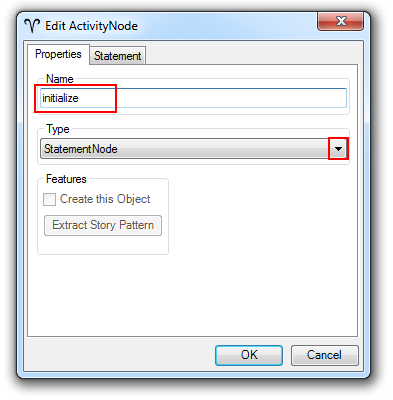
\includegraphics[width=0.5\textwidth]{ea_newStatementNode}
        \label{ea:newStatementNode}
      }
      \subfloat[Edit the \texttt{MethodCallExpression} ]{
        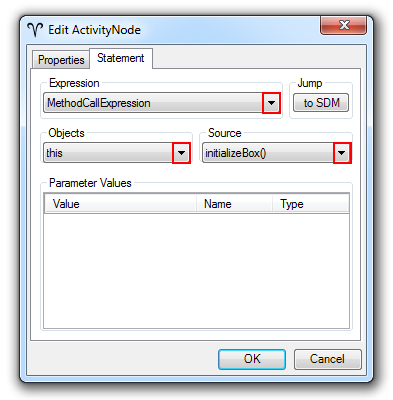
\includegraphics[width=0.5\textwidth]{ea_statementMCExpression}
        \label{ea:statementMCE}
      }
      \caption{}
\end{figure}
\FloatBarrier

\clearpage

\item[$\blacktriangleright$] Now we need to update the edge guards stemming from \texttt{add\-New\-Part\-ition\-In\-Box}. Given that we only want to call
\texttt{initializeBox} if the pattern fails, change the edge guard leading to your statement node to \texttt{Failure}. Similarly, update the edge guard
returning \texttt{true} to \texttt{Success}.

\item[$\blacktriangleright$] Finally, attach two stop nodes -- \texttt{true} and \texttt{false} -- along with their appropriate edge guards from
\texttt{initialize}. These indicate that if the method execution worked, the box could be initialized. If it failed however, \texttt{box} was
in an invalid state (by e.g., having only one partition) and returns \texttt{false}. Overall, the new additions to \texttt{box.grow()} should resemble
Fig.~\ref{ea:newGrowControl}.

\vspace{0.5cm}

\begin{figure}[htp]
\begin{center}
  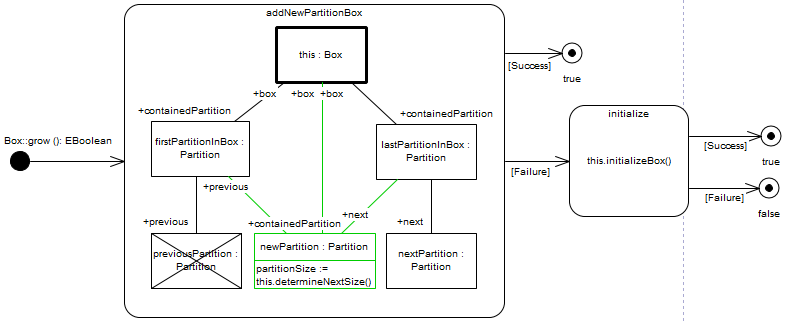
\includegraphics[width=\textwidth]{ea_growAdditions}
  \caption{Extending \texttt{grow} with a \emph{MethodCallExpression}}
  \label{ea:newGrowControl}
\end{center}
\end{figure}

\item[$\blacktriangleright$] To review our work up to this point, we have declared \texttt{initializeBox} and invoked it from a statement node. We have yet
to actually specify the method however. Double-click the anchor to return to the main diagram and create a new SDM
for \texttt{initializeBox}.

\item[$\blacktriangleright$] Create a normal activity node named \texttt{buildPartitions} with the pattern depicted in Fig.~\ref{ea:buildPartitions}.

\newpage
 
\begin{figure}[htp]
\begin{center}
  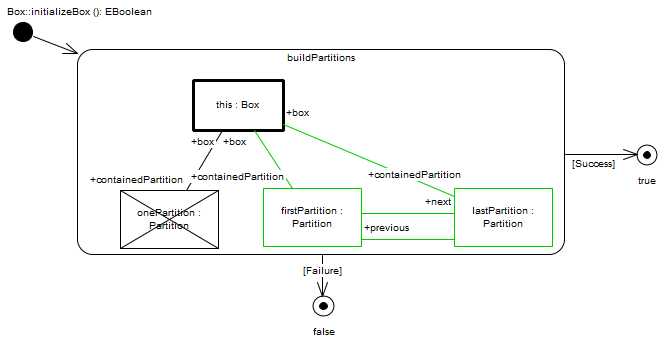
\includegraphics[width=\textwidth]{eclipse_buildPartitions}
  \caption{Complete SDM}
  \label{ea:buildPartitions}
\end{center}
\end{figure}
 
\item[$\blacktriangleright$] The NAC used here is only fulfilled if the box has absolutely no partitions, i.e., is in a pristine state and can be
initialized. In other words, if \texttt{grow} is used for an empty box, it initializes the box for the first time and grows it after that, ensuring that the box
is always in a valid state.
 
\item[$\blacktriangleright$] You're finished! Save, validate, and build your metamodel, then check out how this is done in the textual syntax in
Fig.~\ref{eclipse:updateGrow} and Fig.~\ref{eclipse:pattBuildParts}.

\jumpSingle{initialize notes}

\end{itemize}
